\documentclass[dvipdfmx]{beamer}
\usepackage{mySld}

\begin{document}
\title[OS]{オペレーティングシステム\\第7章 モニタ}
\date{}

\begin{frame}
  \titlepage
\end{frame}

%\begin{frame}
%  \frametitle
%  \tableofcontents
%\end{frame}

\section{概要}
\begin{frame}
  \frametitle{モニタ(Monitor)の概要}

プロセス間同期のために使用できる高級言語の機能のこと.\\
モニタは{\bf 抽象データ型}(Java言語のクラスのようなもの)である.

\begin{itemize}
\item プログラマが定義できる型である.(抽象データ型で一般的)
\item データと操作をまとめて定義する.(抽象データ型で一般的)
\item 同期のための機能が組込まれている.(モニタ独特)
\end{itemize}
\end{frame}

\begin{frame}
  \frametitle{モニタの模式図}
  \begin{center}
    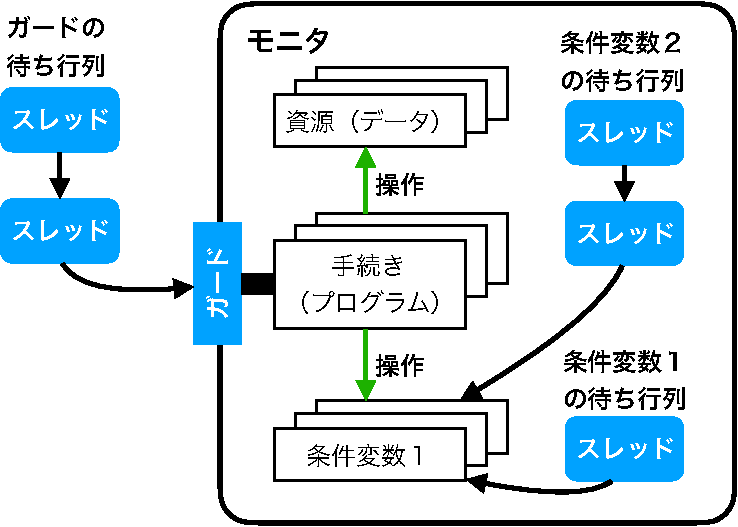
\includegraphics[scale=0.6]{Fig/monitor-crop.pdf}
  \end{center}
  \begin{itemize}
  \item 資源(データ,変数),手続き(メソッド),ガード,条件変数
  \item 図では省略してあるが{\bf 初期化プログラム}
  \end{itemize}
\end{frame}

\section{構成要素}
\begin{frame}
  \frametitle{モニタの構成要素}
\begin{description}
\item [資源(データ、変数)]
複数のスレッドによって共有される変数のことである.
モニタの外から直接アクセスすることはできない.

\item [手続き(操作,メソッド)]
外部から呼び出されるプログラムである.
手続きの実行は{\bf ガード}の働きにより排他的に行われ,
同時に実行される手続きは必ず一つ以内である.

\item [ガード]
モニタに一つのガードが存在し,
手続きを排他的に実行するために用いられる.

\item [条件変数]
条件変数にはwaitとsignalの二つの操作ができる.
wait操作を行ったスレッドは{\bf ガードを外して}条件変数の待ち行列に入る.
signal操作は条件変数の待ち行列から一つのスレッドを選んで実行可能にする.
%実行可能になったスレッドは{\bf ただちに}実行を再開する.
%待ち行列にスレッドが複数ある時,
%どのスレッドが実行可能になるか明確な決まりはない.

\item [初期化プログラム]
モニタのインスタンスを作成する時に,
初期化のために実行されるプログラムである.
\end{description}
\end{frame}

\section{相互排除問題の解}
\begin{frame}
  \frametitle{共有変数を表現するモニタの例(仮想言語)}
  \lstinputlisting{Lst/MonAccount.jama}

  \begin{itemize}
  \item {\bf 資源}はスレッド間の共有変数{\tt money}である.
  \item {\bf 初期化プログラム}はモニタのインスタンス生成時に実行される.
  \item {\bf 手続き}(クリティカルセクション)は,
    ガードにより自動的に相互排除される.
  \end{itemize}
\end{frame}

\begin{frame}
  \frametitle{モニタで表現された共有変数を利用する(仮想言語)}
  \lstinputlisting{Lst/MonAccountMain.jama}

  \begin{itemize}
  \item モニタのインスタンスを生成し,それに対して操作する.
  \item ガードは自動的なので排他忘れが無い.
  \end{itemize}
\end{frame}

\begin{frame}
  \frametitle{セマフォを用いた相互排除問題の解(参考)}
  \lstinputlisting{Lst/semMutex.c}

  \begin{itemize}
  \item P操作とV操作の使用はプログラマまかせ.
  \item 間違うとタイミング異存の発見の難しいバグになる.
  \end{itemize}
\end{frame}

\section{生産者と消費者の問題の解}
\begin{frame}
  \frametitle{モニタによるキューの実現(仮想言語、前半)}
  \lstinputlisting{Lst/BoundedBuffer.jama1}

  \begin{itemize}
  \item この例ではリングバッファのデータ構造が資源である.
  \item 資源はモニタ外部から直接アクセスすることはできない.
  \item 条件変数{\tt empty}はキューが空の時,消費者スレッドが待合せに使用.
  \item 条件変数{\tt full}はキュー満杯時に,生産者者スレッドが待合せに使用.
  \end{itemize}
\end{frame}

\begin{frame}
  \frametitle{モニタによるキューの実現(仮想言語、後半)}
  \lstinputlisting{Lst/BoundedBuffer.jama2}

  \begin{itemize}
  \item {\tt wait()}はスレッドを状態変数の待ち行列に入れる.
  \item {\tt signal()}は状態変数の待ちスレッドを起こす.
  \item {\tt signal()}で起床したスレッドは{\bf ただちに}実行される.
  \end{itemize}
\end{frame}

\begin{frame}
  \frametitle{モニタによる生産者と消費者の問題の解(仮想言語)}
  \lstinputlisting{Lst/BoundedBufferMain.jama}

  \begin{itemize}
  \item モニタにより定義されたキューのインスタンスを使用した解
  \end{itemize}
\end{frame}

\section{セマフォによるモニタの実装}
\begin{frame}
  \frametitle{モニタと同等なキューをJavaのセマフォで実現(1/4)}
  \lstinputlisting{Lst/SemBoundedBuffer.java11}

  \begin{itemize}
  \item Javaのセマフォはカウンティングセマフォ(計数セマフォ)
  \item P操作:{\tt acquireUninterruptibly()},V操作:{\tt release()}
  \end{itemize}
\end{frame}

\begin{frame}
  \frametitle{モニタと同等なキューをJavaのセマフォで実現(2/4)}
  \lstinputlisting{Lst/SemBoundedBuffer.java12}

  \begin{itemize}
  \item 条件変数型を内部クラスとして定義
  \item {\tt wait()}の代わりに{\tt await()}を定義
  \item {\tt exitProc()}は{\bf 手続き}の最後で呼出す.
  \end{itemize}
\end{frame}

\begin{frame}
  \frametitle{モニタと同等なキューをJavaのセマフォで実現(3/4)}
  \lstinputlisting{Lst/SemBoundedBuffer.java21}

  \begin{itemize}
  \item {\bf 資源}はクラス外から見えないように{\tt private}にする.
  \item 前半で宣言した{\bf 条件変数型}の変数を二つ使用.
  \item {\bf 初期化プログラム}はクラスのコンストラクタで実現.
  \end{itemize}
\end{frame}

\begin{frame}
  \frametitle{モニタと同等なキューをJavaのセマフォで実現(4/4)}
  \lstinputlisting{Lst/SemBoundedBuffer.java22}

  \begin{itemize}
  \item モニタなら自動的に実行されるものも明示
  \end{itemize}
\end{frame}

\section{Javaのモニタ風機構による生産者と消費者の問題の解(前半)}
\begin{frame}
  \frametitle{Javaによる生産者と消費者の問題の解(前半)}
  \lstinputlisting{Lst/MonBoundedBuffer.java1}

  \begin{itemize}
  \item 資源には{\tt private}を明示
  \item 初期化はコンストラクタにより実現
  \item Javaの{\tt wait()}はtry-catch構文で使用する必要がある.
  \end{itemize}
\end{frame}

\begin{frame}
  \frametitle{Javaによる生産者と消費者の問題の解(後半)}
  \lstinputlisting{Lst/MonBoundedBuffer.java2}

  \begin{itemize}
  \item {\bf 手続き}は{\tt synchronized}修飾したメソッド
  \item Javaの{\tt wait()}は別の理由でも終了するので{\tt while}の中で使用
  \item 条件変数は一つしかないので,利用方法に工夫が必要
  \item {\tt remove()}最後の行の実行順序がモニタと異なる.
  \end{itemize}
\end{frame}

\end{document}
